\documentclass[]{beamer}

\mode<presentation>{


%%%% ТЕМЫ %%%%
% \usetheme{Berlin} %++main++
% \usetheme{Boadilla} %+
% \usetheme{CambridgeUS} %-
% \usetheme{Madrid} %+
% \usetheme{Frankfurt}
% \usetheme{Montpellier} % свобода в названиях, секциях и подсекциях
% \usetheme{Pittsburgh} %минимализм
\usetheme{Szeged} %классический, без авторов, с нижней строкой


%%%% ЦВЕТА %%%%
% \usecolortheme{beaver} %+осень
% \usecolortheme{crane} %+осень?
% \usecolortheme{dolphin}
% \usecolortheme{dove} %+беленький
% \usecolortheme{seagull} %+business
\usecolortheme{seahorse} %+winter
% \usecolortheme{whale} %+winter
% \usecolortheme{spruce} %+spring


%%%% ДРУГИЕ НАСТРОЙКИ %%%%
%\setbeamertemplate{footline} % To remove the footer line in all slides uncomment this line
%\setbeamertemplate{footline}[frame number] % To replace the footer line in all slides with a simple slide count uncomment this line
\setbeamertemplate{navigation symbols}{} % Чтобы удалить символы навигации со дна всех скользких скользких
% \setbeamercovered{transparent} % Раскрывает серые анимации (полезные для дизайна, но могут быть прокомментированы при передаче окончательного документа)
% Использовать шрифт вспышки везде
\usefonttheme{serif}
}

% \usepackage{graphicx}% Include figure files
\usepackage{dcolumn}% Align table columns on decimal point
\usepackage{bm}% bold math
\usepackage{hyperref}% add hypertext capabilities
% \usepackage{xcolor}

\usepackage{listings} % insert code fragments




\usepackage[T2A]{fontenc}                   %!? закрепляет внутреннюю кодировку LaTeX
\usepackage[utf8]{inputenc}                 %!  закрепляет кодировку utf8
\usepackage[russian, english]{babel}         %!  подключает русский и английский
\usepackage[margin=1.8cm]{geometry}         %!  фиксирует оступ на 2cm

% \usepackage[unicode, pdftex]{hyperref}      %!  оглавление для панели навигации по PDF-документу + гиперссылки

\usepackage{amsthm}                         %!  newtheorem и их сквозная нумерация
\usepackage{hypcap}                         %?  адресация на картинку, а не на подпись к ней
% \usepackage{caption}                        %-  позволяет корректировать caption 
\usepackage{fancyhdr}                       %   добавить верхний и нижний колонтитул
\usepackage{wrapfig}                        %!  обтекание таблиц и рисунков

\usepackage{amsmath}                        %!  |
\usepackage{amssymb,textcomp, esvect,esint} %!  |важно для формул 
\usepackage{amsfonts}                       %!  математические шрифты
\usepackage{mathrsfs}                       %  добавит красивые E, H, L
\usepackage{ulem}                           %!  перечеркивание текста
\usepackage{abraces}                        %?  фигурные скобки сверху или снизу текста
\usepackage{pifont}                         %!  нужен для крестика
\usepackage{cancel}                         %!  аутентичное перечеркивание текста
\usepackage{esvect}                         %  добавит вектора стрелочками

\usepackage{graphicx}                       %?  графическое изменение текста
\usepackage{indentfirst}                    %   добавить indent перед первым параграфом
\usepackage{xcolor}                         %   добавляет цвета
\usepackage{enumitem}                       %!  задание макета перечня.

\usepackage{booktabs}                       %!  добавляет книжные линии в таблицы
% \usepackage{multirow}                       %   объединение ячеек в таблицах
% \usepackage{tikz}                           %!  высокоуровневые рисунки (кружочек)
% \usepackage{import}                         %   |
% \usepackage{xifthen}                        %   |
% \usepackage{pdfpages}                       %   | вставка рисунков pdf_tex
% \usepackage{transparent}                    %   |

\usepackage{bbm}                            %   добавляет \mathbbm{1}


% базовая подстройка
\renewcommand{\d}{\, d}
\renewcommand{\leq}{\leqslant}
\renewcommand{\geq}{\geqslant}


% tmp
\newcommand{\tn}[1]{(\textbf{#1})}
\newcommand{\nBF}{n_\text{\scalebox{0.7}{BF}}}
\newcommand{\Hc}{\sub{h}{c}}
\newcommand{\Z}{\mathcal{Z}}
\newcommand{\Kc}{\sub{K}{c}}
\newcommand{\gs}{\ket{\textnormal{gs}}}
\newcommand{\F}{\mathcal{D}}

% авторские команды
\newcommand{\vc}[1]{\boldsymbol{#1}}
\newcommand{\1}{\mathbbm{1}}
\newcommand{\T}{^{\textnormal{T}}}
\newcommand{\D}{^{\dag}}
\newcommand{\sub}[2]{#1_{\textnormal{#2}}}
\newcommand{\vp}{\vphantom{\dfrac{1}{2}}}
\newcommand{\hc}{\textnormal{h.c.}}

% операторы (просто прямой текст)
\renewcommand{\Im}{\mathop{\mathrm{Im}}\nolimits}
\renewcommand{\Re}{\mathop{\mathrm{Re}}\nolimits}
% \renewcommand{\P}{\mathop{\mathrm{P}}\nolimits}
% \newcommand{\E}{\mathop{\mathrm{E}}\nolimits}
% \newcommand{\D}{\mathop{\mathrm{D}}\nolimits}
% \newcommand{\cov}{\mathop{\mathrm{cov}}\nolimits}
\newcommand{\diag}{\mathop{\mathrm{diag}}\nolimits}
\newcommand{\card}{\mathop{\mathrm{card}}\nolimits}
\newcommand{\grad}{\mathop{\mathrm{grad}}\nolimits}
\renewcommand{\div}{\mathop{\mathrm{div}}\nolimits}
\newcommand{\rot}{\mathop{\mathrm{rot}}\nolimits}
\newcommand{\Ker}{\mathop{\mathrm{ker}}\nolimits}
\newcommand{\spec}{\mathop{\mathrm{spec}}\nolimits}
\newcommand{\sign}{\mathop{\mathrm{sign}}\nolimits}
\newcommand{\tr}{\mathop{\mathrm{tr}}\nolimits}
\newcommand{\rg}{\mathop{\mathrm{rg}}\nolimits}
\newcommand{\const}{\textnormal{const}}


\renewcommand{\th}{\mathop{\mathrm{tanh}}\nolimits}
\newcommand{\sh}{\mathop{\mathrm{sinh}}\nolimits}
\newcommand{\ch}{\mathop{\mathrm{cosh}}\nolimits}

% цветной текст
\newcommand{\red}[1]{\textcolor{red}{#1}}
\newcommand{\green}[1]{\textcolor{urlcolor}{#1}}
\newcommand{\blue}[1]{\textcolor{ublue}{#1}}


% символы
\newcommand{\cmark}{\text{\ding{51}}}
\newcommand{\xmark}{\text{\ding{55}}}


% подгрузка pdf_tex картинок
% \newcommand{\incfig}[1]{%
%     \def\svgwidth{\columnwidth}
%     \import{./figures/}{#1.pdf_tex}
% }


% специфично к квантам
\newcommand{\ket}[1]{\left| #1 \right\rangle}
\newcommand{\bra}[1]{\left\langle #1 \right|}

% \newcommand{\dppp}{\frac{d^3 p}{(2 \pi \hbar)^3}}

\DeclareDocumentCommand{\bk}{m o m}{
    \IfNoValueTF{#2}{\langle #1 | #3 \rangle}{\langle #1 | #2 | #3 \rangle}
}

\DeclareDocumentCommand{\kb}{m o m}{
    \IfNoValueTF{#2}{| #1 \rangle \langle #3 |}{| #1 \rangle #2 \langle #3 |}
}


% снимаю шляпу
% \renewcommand{\hat}[1]{#1}
% % \newif\ifbeamer@tree@showhooks
% \beamer@tree@showhookstrue

% \DeclareOptionBeamer{hooks}[true]{\csname beamer@tree@showhooks#1\endcsname}
% \ProcessOptionsBeamer

% \mode<presentation>
% \defbeamertemplate*{headline}{tree theme}
% {%
%     \begin{beamercolorbox}[wd=\paperwidth,colsep=1.5pt]{upper separation line head}
%     \end{beamercolorbox}
%     \begin{beamercolorbox}[wd=\paperwidth,ht=2.5ex,dp=1.125ex,%
%       leftskip=.3cm,rightskip=.3cm plus1fil]{title in head/foot}
%       \usebeamerfont{title in head/foot}\insertshorttitle
%     \end{beamercolorbox}
%     \begin{beamercolorbox}[wd=\paperwidth,ht=2.5ex,dp=1.125ex,%
%       leftskip=.3cm,rightskip=.3cm plus1fil]{section in head/foot}
%       \usebeamerfont{section in head/foot}%
%       \ifbeamer@tree@showhooks
%         \setbox\beamer@tempbox=\hbox{\insertsectionhead}%
%         \ifdim\wd\beamer@tempbox>1pt%
%           \hskip2pt\raise1.9pt\hbox{\vrule width0.4pt height1.875ex\vrule width 5pt height0.4pt}%
%           \hskip1pt%
%         \fi%
%       \else%  
%         \hskip6pt%
%       \fi%
%       \insertsectionhead
%     \end{beamercolorbox}
%     \begin{beamercolorbox}[wd=\paperwidth,ht=2.5ex,dp=1.125ex,%
%       leftskip=.3cm,rightskip=.3cm plus1fil]{subsection in head/foot}
%       \usebeamerfont{subsection in head/foot}%
%       \ifbeamer@tree@showhooks
%         \setbox\beamer@tempbox=\hbox{\insertsubsectionhead}%
%         \ifdim\wd\beamer@tempbox>1pt%
%           \hskip9.4pt\raise1.9pt\hbox{\vrule width0.4pt height1.875ex\vrule width 5pt height0.4pt}%
%           \hskip1pt%
%         \fi%
%       \else%  
%         \hskip12pt%
%       \fi%
%       \insertsubsectionhead
%     \end{beamercolorbox}
%     \begin{beamercolorbox}[wd=\paperwidth,colsep=1.5pt]{lower separation line head}
%     \end{beamercolorbox}
% }

  
% \mode
% <all>





\newcommand{\progressbar}{% 
	\pgfmathsetmacro{\slidewidth}{\paperwidth}
	\pgfmathsetmacro{\progressstep}{\paperwidth/\inserttotalframenumber}
	\pgfmathsetmacro{\progresspos}{(\insertframenumber - 0.5) * \progressstep}
	\begin{tikzpicture}[scale = 0.035, line width = 1ex]
		\node[inner sep=0pt] (cat) at (\progresspos,0)	{
\includegraphics[width=30pt]{settings/cats/cat_red.pdf}};
		\path[red] (0,0) -- (\slidewidth,0);
	\end{tikzpicture}
}

\makeatletter
\setbeamertemplate{footline}
{
\hfill 
% \progressbar %включить котика
    \leavevmode%
    \hbox{
    \begin{beamercolorbox}[wd=.33\paperwidth,ht=2.25ex,dp=1ex,center]{section in head/foot}
        \insertshortauthor~~\beamer@ifempty{\insertshortinstitute}{}{(\insertshortinstitute)} % раскомментить для авторов
        % \insertshortinstitute % раскомментить для вуза
    \end{beamercolorbox}%
    \begin{beamercolorbox}[wd=.33\paperwidth,ht=2.25ex,dp=1ex,center]{section in head/foot}
        % \insertshortdate{}
        \insertshorttitle
    \end{beamercolorbox}%
    \begin{beamercolorbox}[wd=.33\paperwidth,ht=2.25ex,dp=1ex,right]{section in head/foot}%
        \insertframenumber/\inserttotalframenumber \hspace{1mm}
    \end{beamercolorbox}
    }%
}

%
% \usebeamerfont{author in head/foot}\insertshortauthor~~\beamer@ifempty{\insertshortinstitute}{}{(\insertshortinstitute)} % раскомментить для авторов
% \usebeamerfont{author in head/foot}\beamer@ifempty{\insertshortinstitute}{}{\insertshortinstitute}
% \usebeamerfont{title in head/foot}\insertshorttitle
%   % \usebeamerfont{date in head/foot}\insertshortdate{}\hspace*{2em}
%   % \insertframenumber{} / \inserttotalframenumber\hspace*{2ex} 
% \insertshortinstitute \insertframenumber/\inserttotalframenumber


%%% Логотип
% \usepackage{tikz}
% \addtobeamertemplate{headline}{}{%
% \begin{tikzpicture}[remember picture,overlay]
% \node at([shift={(5.5,-0.5)}]current page.north) {\includegraphics[height=.8\headheight]{settings/cat.png}};
% \end{tikzpicture}}



%%% добавить сетку %%%
% \setbeamertemplate{background}{\tikz[overlay, remember picture, help lines]{
%     \foreach \x in {0,...,12} \path (current page.south west) +(\x,0.5) node {\small$\x$};
%     \foreach \y in {0,...,9} \path (current page.south west) +(0.5,\y) node {\small$\y$};
%     \foreach \x in {0,0.5,...,12.5} \draw (current page.south west) ++(\x,0) -- +(0,9.6);
%     \foreach \y in {0,0.5,...,9.5} \draw (current page.south west) ++(0,\y) -- +(12.8,0);
%   }
% }


%%% верхняя полоска с точками %%%
\setbeamertemplate{headline}
{%
  % \begin{beamercolorbox}[colsep=1.5pt]{upper separation line head}
  % \end{beamercolorbox}
  \begin{beamercolorbox}{section in head/foot}
    \vskip0pt\insertnavigation{\paperwidth}\vskip2pt
  \end{beamercolorbox}%
  \begin{beamercolorbox}[colsep=1.5pt]{lower separation line head}
  \end{beamercolorbox}
}
% \setbeamertemplate{headline}{}


%%% добавить маленькие номера слайдов справа снизу %%%
% \addtobeamertemplate{navigation symbols}{}{%
%     \usebeamerfont{footline}%
%     \usebeamercolor[myred]{footline}%
%     \hspace{1em}%
%     \insertframenumber/\inserttotalframenumber
% }




\setbeamertemplate{frametitle}{%
    \nointerlineskip%
    \begin{beamercolorbox}[wd=\paperwidth,ht=2.0ex,dp=0.6ex]{frametitle}
        \hspace*{1ex}\insertframetitle%
    \end{beamercolorbox}%
}
% set skip of equation length 

\setlength{\abovedisplayskip}{3pt}
\setlength{\abovedisplayshortskip}{3pt}
\setlength{\belowdisplayskip}{3pt}
\setlength{\belowdisplayshortskip}{3pt}
\setlength{\headheight}{13pt}

% \numberwithin{equation}{section}

% \renewcommand{\thesubsection}{\thesection.\alph{subsection}}



\title[Etanglement]{Entanglement}

\author{
Khoruzhii K.}
\institute[MPQ]

\begin{document}
\date{05.07.2024}
\maketitle

% \frame{
% The investigation of quantum phase transitions in strongly correlated systems is an important and fascinating area of research. The one-dimensional Bose-Hubbard model is a minimal bosonic many-particle model that captures the essential physics of interacting bosons on a lattice \cite{kuehner_phases_1998}
\begin{equation*}
	H = -t \sum_{j} (a_j\D a_{j+1} + \hc) + \tfrac{1}{2}U \sum_j n_j (n_j-1) - \mu \sum_j n_j
\end{equation*}
and garnered significant attention due to the existence of both the Mott insulator (MI) and superfluid (SF) phases, as well as the successful application of DMRG \cite{PhysRevLett.69.2863}.

The MI\textsuperscript{\footnote{
    The MI phase is particularly notable for its role in ultracold atom experiments, where it facilitates the deterministic preparation of a single-site occupancy lattice—a critical step in quantum simulation and computation experiments \cite{choi_exploring_2016}.
}} phase is characterized by its lack of particle mobility due to strong interactions, resulting in a fixed integer number of particles per site and an energy gap for particle-hole excitations. This phase exhibits suppressed number fluctuations and localized particles, leading to short correlation lengths and an insulating behavior. In the MI phase, the correlation function $\Gamma(r) = \langle a_j^\dagger a_{j+r} \rangle$ decays \textit{exponentially} with distance (fig. \ref{fig:decay}.1). 

On the other hand, the SF phase features delocalized particles that can move freely across the lattice, leading to long-range phase coherence and the absence of an energy gap. This phase is marked by large number fluctuations and a diverging correlation length, indicating a coherent, macroscopic quantum state. In the SF phase, the correlation function $\Gamma(r)$ decays \textit{polynomially} with distance (fig. \ref{fig:decay}.3).


\begin{figure}[b]
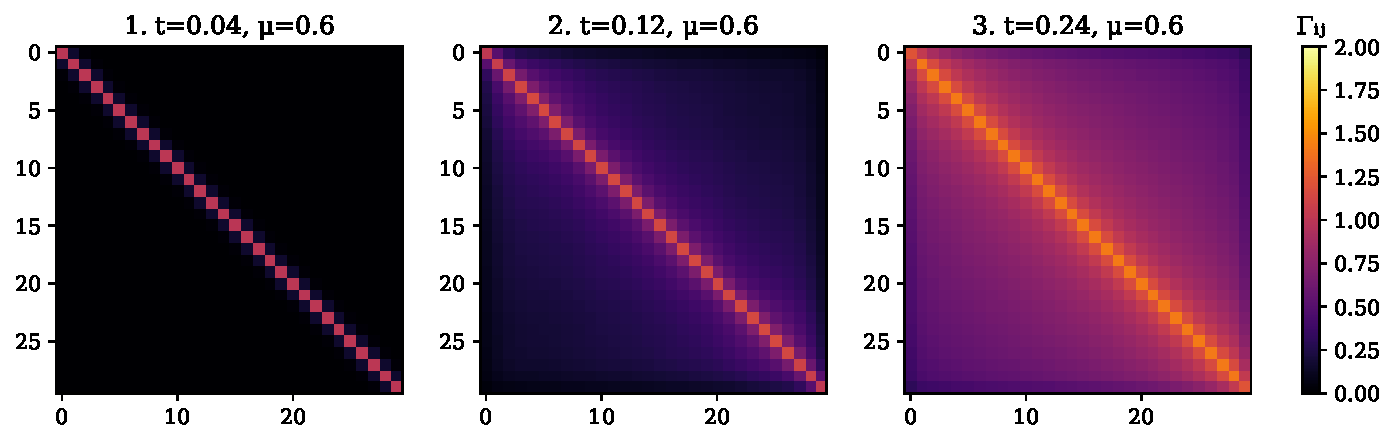
\includegraphics[width=\linewidth]{imgs/corrs.pdf}
\caption{The characteristic form of $\Gamma_{ij}$ at three points in the phase space: MI (1), critical point (2), and SF (3). The same points are used for illustration purposes throughout the text.}
\label{fig:corrmat}
\end{figure}

\section{Methodology}


In this article, we will focus on three key quantities to distinguish between these phases: the correlation length $\xi$, the average site occupancy $\langle n_j \rangle$, and the polynomial degree \( K \) with which \(\Gamma^2\) decays, following the approach in [1]. These properties provide valuable insights into the nature of the MI and SF phases. By examining these parameters, we aim to deepen our understanding of the phase transitions within the one-dimensional Bose-Hubbard model.




 \frametitle{Intro}}

\frame{
 \begin{tikzpicture}[overlay, remember picture]
        \node[circle, fill=black, inner sep=2pt, label=above:$A$] at (current page.north east) [xshift=-2cm, yshift=-2cm] (A) {};
        \node[circle, fill=black, inner sep=2pt, label=above:$B$] at (current page.north east) [xshift=-1cm, yshift=-2cm] (B) {};
        \draw (A) -- (B);
\end{tikzpicture}



\begin{itemize}
    \iitem  Pure states $\ket{\psi_{AB}}$: 
        \begin{itemize}
            \iitem{\textit{Product state} if $\ket{\psi_{AB}} = \ket{\psi_A} \otimes \ket{\psi_B}$}
            \iitem{$A$ is entangled with $B$ otherwise}
        \end{itemize}
    \vspace{3mm}
    \iitem Mixed states $\hat{\rho}_{AB}$
    \begin{itemize}
        \iitem{\textit{Separable state} if $\hat{\rho}_{AB} = \sum_k p_k \hat{\rho}_A^k \otimes \hat{\rho}_B^k$}
        \iitem{$A$ is entangled with $B$ otherwise}
    \end{itemize}
\end{itemize}

\vfill

\begin{figure}[h]
    \centering
    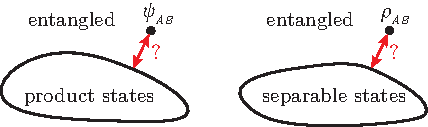
\includegraphics{imgs/Asset 2.pdf}
    %\caption{}
    %\label{fig:}
\end{figure}


% \begin{minipage}{0.45\textwidth}
%     \begin{block}{Entangled}
        
%     \end{block}
% \end{minipage}
% \hfill
% \begin{minipage}{0.45\textwidth}
%     \begin{block}{Non-entangled states}
%         For pure states: 
%     \end{block}
% \end{minipage}
%      \frametitle{States}}


\frame{
 \begin{tikzpicture}[overlay, remember picture]
        \node[circle, fill=black, inner sep=2pt, label=above:$A$] at (current page.north east) [xshift=-2cm, yshift=-2cm] (A) {};
        \node[circle, fill=black, inner sep=2pt, label=above:$B$] at (current page.north east) [xshift=-1cm, yshift=-2cm] (B) {};
        \draw (A) -- (B);
\end{tikzpicture}


\only<1,2>{
    \onslide<1,2>{
        Is this state entangled?
        \begin{equation*}
            \ket{\psi_{AB}} = \tfrac{1}{\sqrt{2}}\left(\ket{00} + \ket{01}\right)
        \end{equation*}
    }
    \onslide<2>{
    Of course not:
    \begin{equation*}
        \ket{\psi_{AB}} = \ket{0} \otimes \frac{1}{\sqrt{2}} \left(\ket{0}+ \ket{1}\right)
    \end{equation*}
    }
}
\only<3,4,5,6>{
    \onslide<3,4,5,6>{
    What about this?
    \begin{equation*}
        \ket{\psi_{AB}} = \tfrac{1}{2}\left(\ket{00} + \ket{10} - \ket{01} - \ket{11}\right)
    \end{equation*}
    }
    \onslide<4,5,6>{
    After some SVD (or \textbf{Schmidt decomposition}):
    \begin{equation*}
        \ket{\psi_{AB}} = \sum_{a \in A} \sum_{b \in B} \psi_{ab} \ket{a} \otimes \ket{b} = \sum_a \sum_b \frac{1}{2}\begin{pmatrix}
        1 & -1 \\
        1 & -1 \\
    \end{pmatrix}_{ab}
     \ket{ab}
    \end{equation*}
    }
    \only<5>{
        \begin{equation*}
        U \begin{pmatrix}
            \sqrt{\lambda_1} & 0 \\
            0 & \sqrt{\lambda_2} \\
        \end{pmatrix} V = 
        \frac{1}{\sqrt{2}}\begin{pmatrix}
        1 & . \\
        1 & . \\
        \end{pmatrix}
        \begin{pmatrix}
        1 & 0 \\
        0 & 0 \\
        \end{pmatrix}
        \frac{1}{\sqrt{2}}
        \begin{pmatrix}
        1 & . \\
        -1 & . \\
        \end{pmatrix}
        =
        \frac{1}{2}
        \begin{pmatrix}
        1 & -1 \\
        1 & -1 \\
        \end{pmatrix}       
        \end{equation*}
    }
    \only<6>{
        \begin{equation*}
            \ket{\psi_{AB}} = \tfrac{1}{\sqrt{2}} \left(\ket{0} + \ket{1}\right) \otimes \tfrac{1}{\sqrt{2}} \left(\ket{0} - \ket{1}\right)
        \end{equation*}
        We can see, that it is separable.
    }
}
\only<7>{
    Schmidt decomposition
    \begin{equation*}
        \ket{\psi_{AB}} = \sum_{a \in A} \sum_{b \in B} \psi_{ab} \ket{a} \otimes \ket{b} = \sum_j \sqrt{\lambda_j} \ket{\psi_{A,j}} \ket{\psi_{B,j}}
    \end{equation*}
    feeply connected with the reduced density matrix $\rho_{A,B}$
    \begin{equation*}
        \rho_{B, A} = \tr_{A,B} \left(\ket{\psi_{AB}}\right) = \sum_{i} \lambda_i \kb{\psi_{B,A}}{\psi_{B,A}}.
    \end{equation*}

    If there is no entanglement, than 
    \begin{equation*}
        \rho_{A,B} = \kb{\psi_{A,B}}{\psi_{A,B}} 
    \end{equation*}
} \frametitle{Bipartite entanglement in pure states: SVD}}

\frame{
 \begin{tikzpicture}[overlay, remember picture]
        \node[circle, fill=black, inner sep=2pt, label=above:$A$] at (current page.north east) [xshift=-2cm, yshift=-1.6cm] (A) {};
        \node[circle, fill=black, inner sep=2pt, label=above:$B$] at (current page.north east) [xshift=-1cm, yshift=-1.6cm] (B) {};
        \draw (A) -- (B);
\end{tikzpicture}


\only<1>{
	Which one is more entangled?
}
\only<2, 3, 4>{
	Which one is more entangled? (singular values could help):
}
\begin{align*}
	\onslide<1, 2, 3, 4>{
		\ket{\psi_{AB}^{I}} &= \tfrac{1}{\sqrt{4}}\left(\ket{00} + \ket{10} - \ket{01} - \ket{11}\right), 
	}
	\onslide<2, 3, 4>{
		&\lambda_{1,2}^{I} &= \{1, 0\}
	}
	\\
	\onslide<1, 2, 3, 4>{
		\ket{\psi_{AB}^{II}} &= \tfrac{1}{\sqrt{3}}\left(\ket{00} + \ket{01} + \ket{10}\right), 
	}
	\onslide<2, 3, 4>{
		&\lambda_{1,2}^{II} &= \{0.87, 0.13\}
	}
	\\
	\onslide<1, 2, 3, 4>{
		\ket{\psi_{AB}^{III}} &= \tfrac{1}{\sqrt{2}}\left(\ket{00} + \ket{11}\right) 
	}
	\onslide<2, 3, 4>{
		&\lambda_{1,2}^{III} &= \{0.5, 0.5\}
	}
	\\
\end{align*}

\onslide<3,4>{
Measure of entanglement is fixed, if it has
\begin{itemize}
	\iitem{invariance under LUO $ \Rightarrow E = E(\lambda)$} %local unitary operators
	\iitem{continuity}
	\iitem{additivity $E(\ket{\psi_{AB}} \otimes \ket{\varphi_{AB}}) = E(\ket{\psi_{AB}}) + E(\ket{\varphi_{AB}})$}
\end{itemize}
}

\onslide<4>{
This is \textit{the von Neumann entropy}
\begin{equation*}
\boxed{
	S(\rho_A) = S(\rho_B) = - \sum_j \lambda_j \ln \lambda_j,
}
	\hspace{5 mm} 
	S^{I} = 0, \ 
	S^{II} = 0.6, \ 
	S^{II} = 1.
\end{equation*}
}

% This $\lambda_{1,2}$ from Schmidt decomposition help us to construct nice measure of entanglement: the von Neumann entropy 
% \begin{equation*}
% f	
% \end{equation*} \frametitle{Von Neumann Entropy}}

\frame{
\begin{tikzpicture}[overlay, remember picture]
    \node[anchor=north west, rotate=0, gray, font=\tiny, text width=\paperwidth] at (current page.south west)  [xshift=0, yshift=1.cm] {
    [2] Rajibul Islam et al., Measuring entanglement entropy through the interference of quantum many-body twins, Nature, 528 (2015)
    };
\end{tikzpicture}

\begin{minipage}{0.4\textwidth}

\only<1>{
Sufficient to show:
\begin{align*}
	\tr(\rho_A^2) < \tr(\rho_{AB}^2) \\
	\tr(\rho_B^2) < \tr(\rho_{AB}^2) \\
\end{align*}

\vspace{-5mm}

\begin{figure}[h]
    \centering
    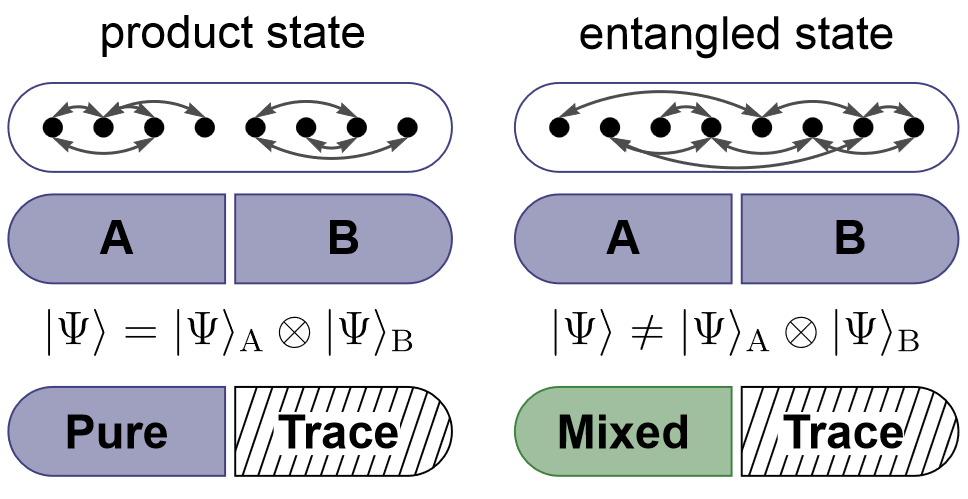
\includegraphics[width=0.95\textwidth]{imgs/int_1.png}
    \vspace{4mm}
    \caption{Bipartite entanglement and partial measurements.}
\end{figure}
}
\only<2>{
\begin{figure}[h]
    \centering
    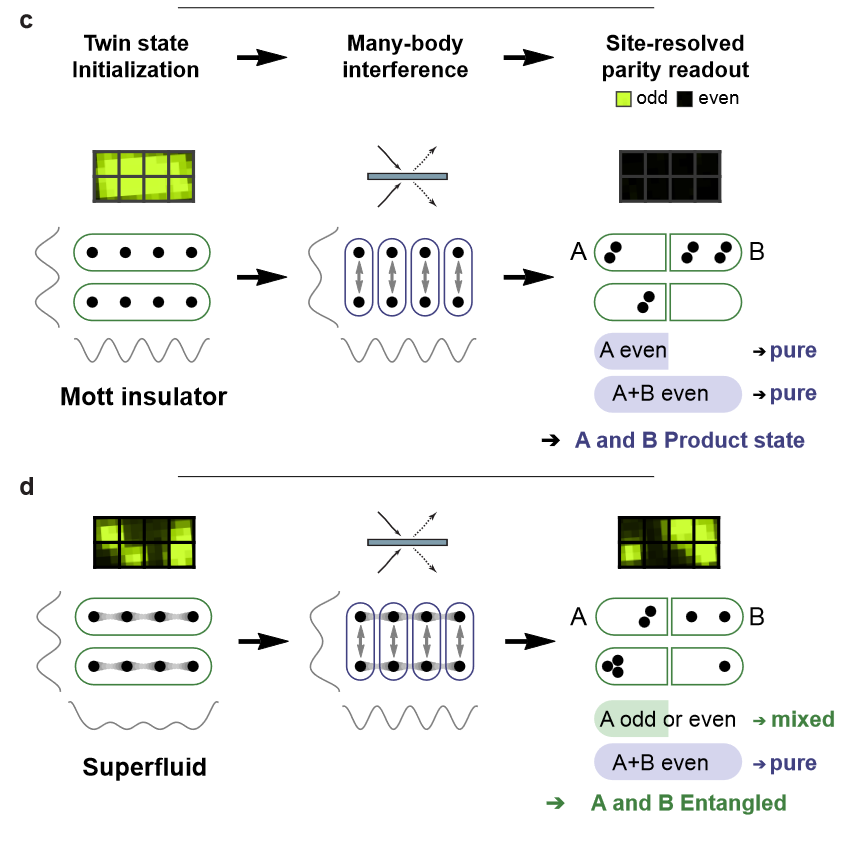
\includegraphics[width=1.1\textwidth]{imgs/int3.png}
    \caption{Many-body interference to probe entanglement in optical lattices}
    %\label{fig:}
\end{figure}

}

\end{minipage}
\hfill
\begin{minipage}{0.5\textwidth}
\begin{figure}[h]
    \centering
    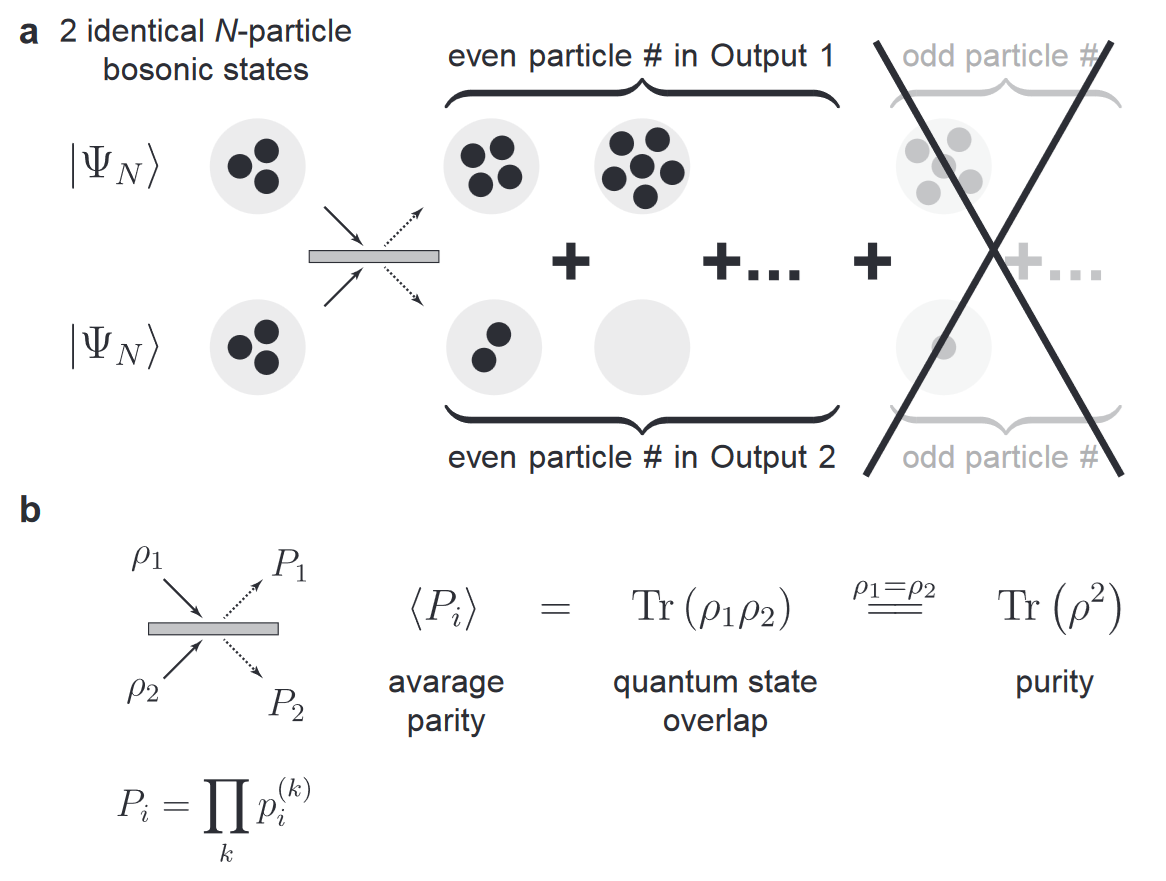
\includegraphics[width=1.0\textwidth]{imgs/int_2.png}
    \vspace{2mm}
    \caption{Measurement of quantum purity with many-body bosonic interference of quantum twins}
\end{figure}
\end{minipage}



 \frametitle{Example of measurement}}

% \frame{
% \begin{tikzpicture}[overlay, remember picture]
    \node[anchor=north west, rotate=0, gray, font=\tiny, text width=\paperwidth] at (current page.south west)  [xshift=0, yshift=0.75cm] {
    [1] L. Amico et al., Entanglement in Many-Body Systems, Reviews of Modern Physics 80, no. 2 (2008)
    };
\end{tikzpicture}

The purity of the state represented by \textit{one-tangle}
\begin{equation*}
	\tau_1[\rho_A] = 4 \det \rho_A = 1 - 4 \left(
		\langle S_x\rangle^2+\langle S_y\rangle^2+\langle S_z\rangle^2
	\right)
\end{equation*}
for $\rho_A = \tr_B \rho_{AB}$.

\phantom{42}

\onslide<2,3>{
For a pure state of \underline{two qubits} we can define \textit{concurrence}
\begin{equation*}
	C[\ket{\psi_{AB}}] = |\bk{\psi^*}[\sigma_A^y \otimes \sigma_B^y]{\psi}| = \sqrt{\tau_1}
\end{equation*}
}

% \phantom{42}

\onslide<3>{
Not all entanglement is stored in pairs:
\begin{equation*}
	\text{residual tangle} = \tau_{1, i} - \sum_{j \neq i} C_{ij}^2 \geq 0
\end{equation*}
} \frametitle{Paired entanglement}}

% \frame{
%  \begin{tikzpicture}[overlay, remember picture]
        \node[circle, fill=black, inner sep=2pt, label=above:$A$] at (current page.north east) [xshift=-2cm, yshift=-1.5cm] (A) {};
        \node[circle, fill=black, inner sep=2pt, label=above:$B$] at (current page.north east) [xshift=-1cm, yshift=-1.5cm] (B) {};
        \draw (A) -- (B);
\end{tikzpicture}

The Entanglement of Formation  defined throught \textit{convex roof}:
\begin{equation*}
	E_F(\rho_{AB}) \overset{\mathrm{def}}{=} \min_{\{p_j, \psi_j\}} \sum_j p_j S(\rho_{A,j}), 
\end{equation*}
with $\rho_{AB} = \sum_j p_j \kb{\psi_j}{\psi_j}$ and $\rho_{A,j} = \tr_B \kb{\psi_j}{\psi_j}$.


\onslide<2>{
	\phantom{42}

	For two qubits:
	\begin{equation*}
		E_F(\rho) = - \sum_{\sigma = \pm} \tfrac{1}{2}\sqrt{1+\sigma C^2(\rho)} \ln \tfrac{1}{2}\sqrt{1 + \sigma C^2(\rho)},
	\end{equation*}
	$C(\rho) \in [0, 1]$ -- \textit{concurrence}, that can be calculated from $R = \sqrt{\rho} \tilde{\rho} \sqrt{\rho} = \sqrt{\rho} (\sigma_y \otimes \sigma_y) \rho^* (\sigma_y \otimes \sigma_y)$ with $\lambda_1^2 \geq \ldots \geq \lambda_4^2$
	\begin{equation*}
		C = \max(\lambda_1 - \lambda_2 - \lambda_3 - \lambda_4, 0).
	\end{equation*}
} \frametitle{Entanglement in mixed states: EoF}}

% \frame{
% \begin{tikzpicture}[overlay, remember picture]
    \node[anchor=north west, rotate=0, gray, font=\tiny, text width=\paperwidth] at (current page.south west)  [xshift=0, yshift=0.75cm] {
    [1] L. Amico et al., Entanglement in Many-Body Systems, Reviews of Modern Physics 80, no. 2 (2008)
    };
\end{tikzpicture}


In a spin-1/2 chain
\begin{equation*}
	C_{ij} = 2 \max\{0,\, C_{ij}^I,\, C_{ij}^{II} \},
\end{equation*}
where 
\begin{align*}
	C_{ij}^I &= |g_{ij}^{xx} + g_{ij}^{yy}| - \sqrt{(1/4 + g_{ij}^{zz})^2 - M_z^2} \\
	C_{ij}^{II} &= |g_{ij}^{xx} - g_{ij}^{yy}| + g_{ij}^{zz} - 1/4,
\end{align*}
with $g_{ij}^{\alpha\alpha} = \langle S_i^\alpha S_j^\alpha\rangle$ and $M_z = \langle S^z\rangle$.


 \frametitle{Concurrence through two-point spin correlation}}

\frame{
\begin{tikzpicture}[overlay, remember picture]
    \node[anchor=north west, rotate=0, gray, font=\tiny, text width=\paperwidth] at (current page.south west)  [xshift=0, yshift=1.5cm] {
    [2] A. Bergschneider et al., Experimental Characterization of Two-Particle Entanglement through Position and Momentum Correlations, Nature Physics 15, no. 7 (2019)

    \only<3,4>{
    [3] M. Jafarpour et al., A Useful Strong Lower Bound on Two-Qubit Concurrence, Quantum Information Processing 11, no. 6 (2012)
    }
    };
\end{tikzpicture}

% Jafarpour, Mojtaba, and Abbass Sabour. ‘A Useful Strong Lower Bound on Two-Qubit Concurrence’. Quantum Information Processing 11, no. 6 (December 2012): 1389–1402. https://doi.org/10.1007/s11128-011-0288-0.


% \begin{figure}[h]
%     \centering
%     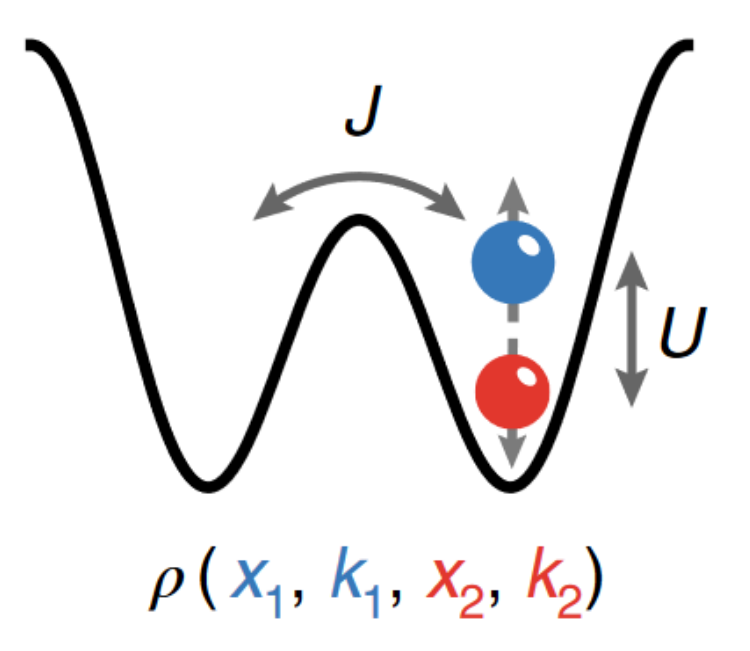
\includegraphics[width=0.5\textwidth]{imgs/Exp1.png}
%     %\caption{}
%     %\label{fig:}
% \end{figure}


% , Andrea, Vincent M. Klinkhamer, Jan Hendrik Becher, Ralf Klemt, Lukas Palm, Gerhard Zürn, Selim Jochim, and Philipp M. Preiss. ‘’. Nature Physics 15, no. 7 (July 2019): 640–44. https://doi.org/10.1038/s41567-019-0508-6.

%  \begin{tikzpicture}[overlay, remember picture]
%         \node[circle, fill=black, inner sep=2pt, label=above:$A$] at (current page.north east) [xshift=-2cm, yshift=-1.5cm] (A) {};
%         \node[circle, fill=black, inner sep=2pt, label=above:$B$] at (current page.north east) [xshift=-1cm, yshift=-1.5cm] (B) {};
%         \draw (A) -- (B);
% \end{tikzpicture}

\only<1>{
Consider dimer system
	\begin{figure}[h]
	    \centering
	    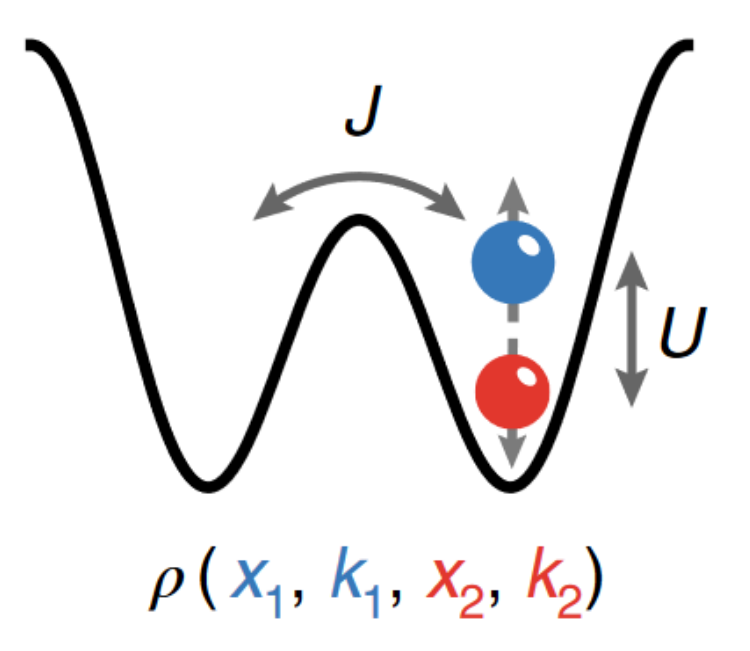
\includegraphics[width=0.3\textwidth]{imgs/Exp1.png}
	    %\caption{}
	    %\label{fig:}
	\end{figure}
With Hamiltonian
}
\only<1,2,3,4>{
\only<2,3,4>{\vspace{-1cm}}
\begin{equation*}
	\hat{H} = - J \sum_\sigma \left(\hat{c}_{\text{L} \sigma} \hat{c}_{\text{R} \sigma} + \text{c.c.}\right) + U \sum_{j=\text{L,R}} \hat{n}_{j \downarrow} \hat{n}_{j \uparrow}
\end{equation*}

% \phantom{42}


}
\only<2,3,4>{
What is available for us to measure?
\begin{minipage}{0.45\textwidth}
\begin{figure}[h]
    \centering
    \only<2,3,4>{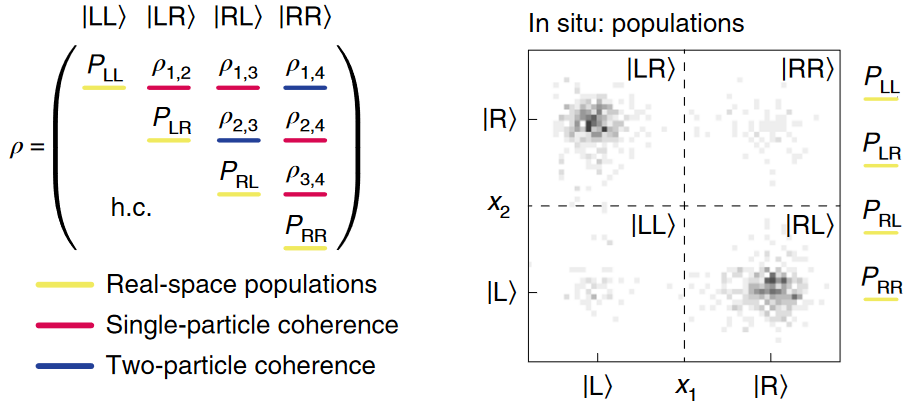
\includegraphics[width=\textwidth]{imgs/Exp4.png}}
    %\caption{}
    %\label{fig:}
\end{figure}
\end{minipage}
\hfill
\begin{minipage}{0.45\textwidth}
\begin{figure}[h]
    \centering
    \only<2,3>{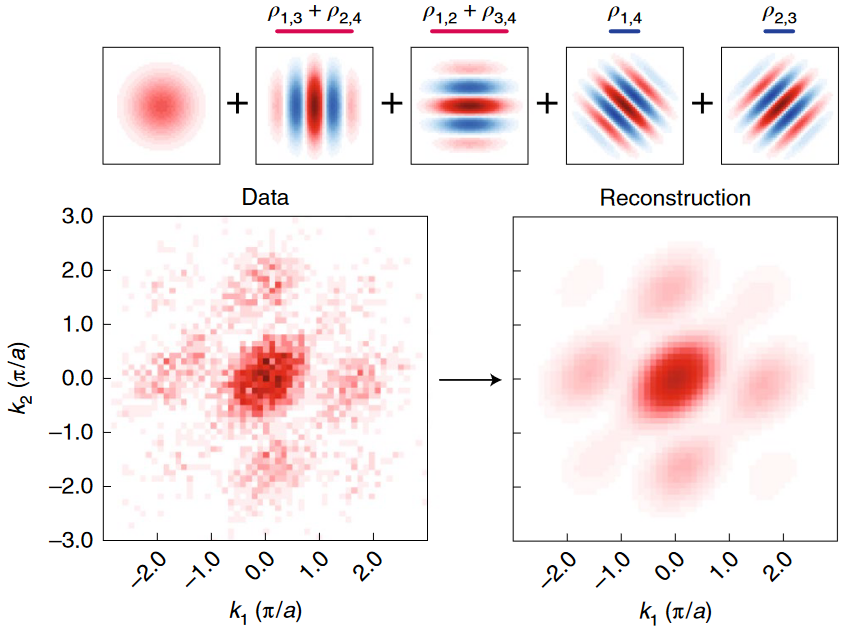
\includegraphics[width=\textwidth]{imgs/Exp2.png}}
    \only<4>{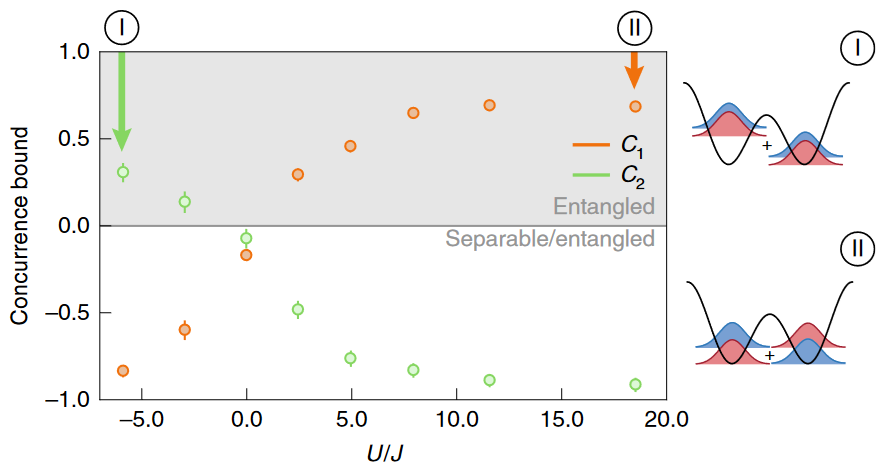
\includegraphics[width=\textwidth]{imgs/Exp3.png}}
    %\caption{}
    %\label{fig:}
\end{figure}
\end{minipage}


\onslide<3,4>{
\only<3>{\vspace{-5mm}}
	Lower bound for concurrence
	\begin{equation*}
		C(\rho) \geq \max\left\{
			0, \
			2(|\rho_{1,4}| - \sqrt{\sub{P}{LR} \sub{P}{RL}}),\
			2(|\rho_{2,3}| - \sqrt{\sub{P}{LL} \sub{P}{RR}})
		\right\}
	\end{equation*}
}

}

 \frametitle{Measurable example}}

% \frame{
% \begin{tikzpicture}[overlay, remember picture]
    \node[anchor=north west, rotate=0, gray, font=\tiny, text width=\paperwidth] at (current page.south west)  [xshift=0, yshift=0.75cm] {
    [1] L. Amico et al., Entanglement in Many-Body Systems, Reviews of Modern Physics 80, no. 2 (2008)
    };
\end{tikzpicture}


\begin{figure}[h]
    \centering
    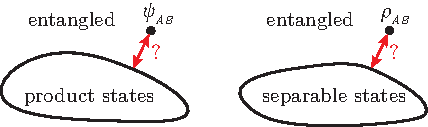
\includegraphics{imgs/Asset 2.pdf}
    %\caption{}
    %\label{fig:}
\end{figure}

\phantom{42}

\onslide<2, 3>{
Measure of entanglement: <<dinstance>> from separable states
\begin{equation*}
    E(\rho) \overset{\mathrm{def}}{=} \min_{\rho' \in \mathcal{D}} S(\rho || \rho'),
\end{equation*}
with = $S(\rho || \rho') = \tr \rho (\ln \rho - \ln \rho')$.
}

\phantom{42}

\onslide<3>{
*reduces to $S(\rho)$ in the case of pure bi-partite states.
} \frametitle{Relative entropy of entanglement}}


% \frame{
% \begin{tikzpicture}[overlay, remember picture]
    \node[anchor=north west, rotate=0, gray, font=\tiny, text width=\paperwidth] at (current page.south west)  [xshift=0, yshift=0.75cm] {
    [1] L. Amico et al., Entanglement in Many-Body Systems, Reviews of Modern Physics 80, no. 2 (2008)
    };
\end{tikzpicture}


\begin{figure}[h]
    \centering
    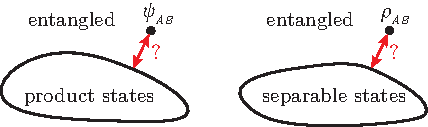
\includegraphics{imgs/Asset 2.pdf}
    %\caption{}
    %\label{fig:}
\end{figure}

\phantom{42}


% \onslide<1>{
\textbf{Multipartite} entanglement: <<dinstance>> from product states \vspace{-2mm}
\begin{equation*}
    E_g(\Psi) \overset{\mathrm{def}}{=} - \log_2 \max_{\Phi \in \mathcal{S}} |\bk{\Psi}{\Phi}|^2,
\end{equation*}
% \phantom{42}
% with = $S(\rho || \rho') = \tr \rho (\ln \rho - \ln \rho')$.
% }


\onslide<2>{
Or average purity  \vspace{-5mm}
\begin{equation*}
    \sub{E}{gl} \overset{\mathrm{def}}{=}  2 - \frac{2}{N} \sum_{j=1}^N \tr \rho_j^2
\end{equation*}
% *reduces to $S(\rho)$ in the case of pure bi-partite states.
} \frametitle{Multipartite entanglement measures}}



\frame{
\begin{tikzpicture}[overlay, remember picture]
    \node[anchor=north west, rotate=0, gray, font=\tiny, text width=\paperwidth] at (current page.south west)  [xshift=0, yshift=1.25cm] {
    [1] L. Amico et al., Entanglement in Many-Body Systems, Reviews of Modern Physics 80, no. 2 (2008)

    [4] A. P. Majtey et al., Indistinguishable Entangled Fermions: Basics and Future Challenges, Phil. Trans. R. Soc. A.381 (2023)
    };
\end{tikzpicture}



Consider state represented by the Slater determinant
\begin{equation*}
	\ket{\psi}^{\text{SD}} = \frac{1}{\sqrt{2}}\left(
		\ket{A,0} \ket{B,1} - \ket{B,1} \ket{A,0}
	\right),
\end{equation*}
with $A,B$ and $0,1$ are the spatial and the internal degree of freedom.

\phantom{42}

\onslide<2,3>{
\only<2>{
This state results from antisymmetrizing the product state
\begin{equation*}
	\ket{\psi}^{\text{prod}} = \ket{A,0} \ket{B,1},
\end{equation*}
so no entanglement actually.
}
\onslide<3>{

	Meanwhile reduced density matrix is inpure
\begin{equation*}
	\rho^{\text{SD}}_\text{f} = \tfrac{1}{2}	\kb{A,0}{A,0} + \tfrac{1}{2} \kb{B,1}{B,1}.
\end{equation*}

}
}

 \frametitle{Indistinguishable particles: example}}

\frame{
\begin{tikzpicture}[overlay, remember picture]
    \node[anchor=north west, rotate=0, gray, font=\tiny, text width=\paperwidth] at (current page.south west)  [xshift=0, yshift=1.25cm] {
    [1] L. Amico et al., Entanglement in Many-Body Systems, Reviews of Modern Physics 80, no. 2 (2008)

    [4] A. P. Majtey et al., Indistinguishable Entangled Fermions: Basics and Future Challenges, Phil. Trans. R. Soc. A.381 (2023)
    };
\end{tikzpicture}

\only<1>{
In general for $N$ identical fermions identified with a single Slater determinant reduced density matrix of $M$ fermions
\begin{equation*}
	\tr \left(\rho_M^{\text{SD}}\right)^2 = \begin{pmatrix}
		N \\ M
	\end{pmatrix}^{-1}.
\end{equation*}
Such correlations are compatible with the possibility of assigning a complete set of properties to the individual fermions.
}

\only<2, 3>{
	
State that can not be represented by the Slater determinant
\begin{gather*}
	\ket{\psi}^{\text{SD}} = \tfrac{1}{2}\left(
		\ket{A,0} \ket{B,1} - \ket{B,1} \ket{A,0} + \ket{A,1} \ket{B,0} - \ket{B,0} \ket{A,1}
	\right), \\
	\ket{\psi}^{\text{non-prod}} = \tfrac{1}{\sqrt{2}}\left(\ket{A,0} \ket{B,1} + \ket{A,1} \ket{B,0}\right)
\end{gather*}
And the purity of $\rho^{\text{non-SD}}_\text{f}$ is lower than the purity of $\rho^{\text{SD}}_\text{f}$.

\phantom{42}

\only<2>{
This feature reveals the presence of correlations beyond exchange correlations.
}
}


\only<3>{
Entanglament criteria: \vspace{-3mm}
	\begin{equation*}
		\tr \rho_M^2 < \begin{pmatrix}
			N \\ M
		\end{pmatrix}^{-1}
		\hspace{5 mm} 
		\Leftrightarrow
		\hspace{5 mm} 
		\ket{\psi} \text{ is entangled}.
	\end{equation*}

In other words: how many Slater determinants you need to describe the state (\textit{Slater rank})?
} \frametitle{Indistinguishable particles: fermionic exchange correlations}}



\frame{
\begin{tikzpicture}[overlay, remember picture]
    \node[anchor=north west, rotate=0, gray, font=\tiny, text width=\paperwidth] at (current page.south west)  [xshift=0, yshift=1.25cm] {
    [4] Adam Nahum et al., Quantum Entanglement Growth Under Random Unitary Dynamics, Physical Review X, 7.3 (2017s)
    };
\end{tikzpicture}

% Quantum Entanglement Growth Under Random Unitary Dynamics:
\vspace{-0.5cm}
\phantom{42} \vspace{-0.5cm}

\begin{figure}[h]
    \centering
    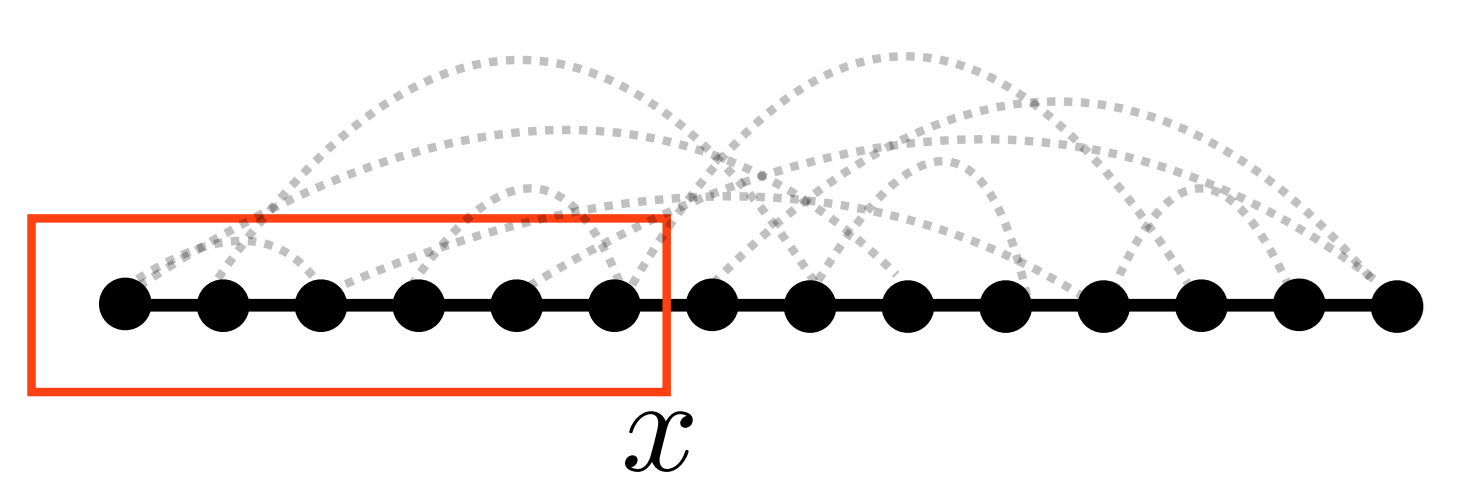
\includegraphics[width=0.4\textwidth]{imgs/guo_2.png}
    %\caption{}
    %\label{fig:}
\end{figure}

\vspace{-1cm}
Renyi entropy:
\begin{equation*}
	S_n(x) = \frac{1}{1-n} \ln(\tr \rho_x^n), 
	\hspace{5 mm} 
	|S(x+1) - S(x)| \leq 1.
\end{equation*}

With random updates \vspace{-4mm}
\begin{figure}[h]
    \centering
    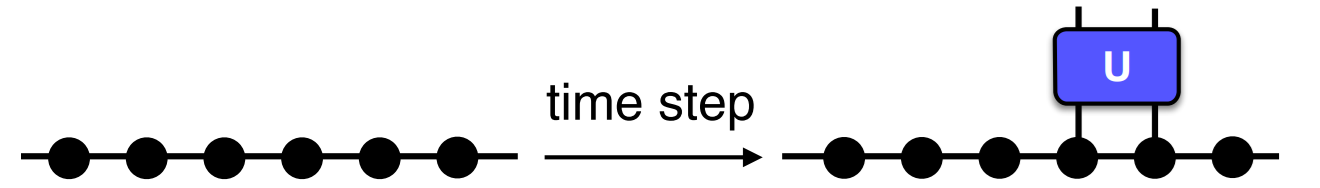
\includegraphics[width=0.5\textwidth]{imgs/guo_1.png}
    %\caption{}
    %\label{fig:}
\end{figure}

\vspace{-0.5cm}
\begin{equation*}
	S_0(x, t+1) = \min[S_0(x-1,t), S_0(x+1,t)] + 1
\end{equation*}

\vspace{-0.5cm}
\begin{figure}[h]
    \centering
    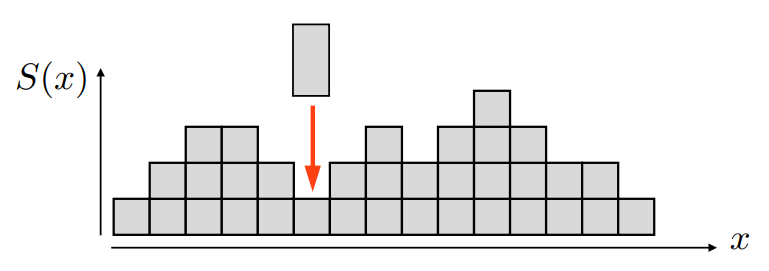
\includegraphics[width=0.5\textwidth]{imgs/guo_3.png}
    % \caption{}
    %\label{fig:}
\end{figure}
 \frametitle{Non-local Unitary Operations}}


% \frame{ %2Do: part transpose & PPTES, exp with corr on product
% \begin{tikzpicture}[overlay, remember picture]
    \node[anchor=north west, rotate=0, gray, font=\tiny, text width=\paperwidth] at (current page.south west)  [xshift=0, yshift=0.75cm] {
    [1] L. Amico et al., Entanglement in Many-Body Systems, Reviews of Modern Physics 80, no. 2 (2008)
    };
\end{tikzpicture}


% \only<1>{
Some property, that differs for separable and entangled states.


\begin{figure}[h]
    \centering
    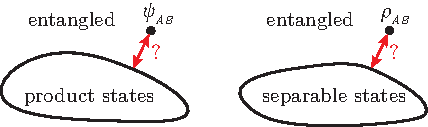
\includegraphics{imgs/Asset 2.pdf}
    %\caption{}
    %\label{fig:}
\end{figure}

% }

\onslide<2,3>{

\phantom{42}

A state $\rho_{AB}$ is entangled if and only if a positive map $\Lambda$ exists: 
\vspace{-2mm}
\begin{equation*}
	\left(\mathbbm{1}_A \otimes \Lambda_B \right) \rho_{AB} < 0.
\end{equation*}

}


\onslide<3>{

% \phantom{42}

Peres-Horodecki criterion of being separable:
\vspace{-2mm}
\begin{equation*}
	\rho_{AB}^{T_B} \geq 0.
\end{equation*}

} \frametitle{Entanglement witnesses}}


% \frame{ %2Do: part transpose & PPTES, exp with corr on product
% \begin{tikzpicture}[overlay, remember picture]
    \node[anchor=north west, rotate=0, gray, font=\tiny, text width=\paperwidth] at (current page.south west)  [xshift=0, yshift=0.75cm] {
    [1] L. Amico et al., Entanglement in Many-Body Systems, Reviews of Modern Physics 80, no. 2 (2008)
    };
\end{tikzpicture}


\only<1,2>{

Peres-Horodecki criterion of being separable (sufficient):
\vspace{-2mm}
\begin{equation*}
    \rho_{AB}^{T_B} \geq 0.
\end{equation*}
\vspace{-5mm}


% \phantom{42}

\begin{minipage}{0.55\textwidth}
    Necessary for:
    \begin{itemize}
        \iitem{two qubits}
        \iitem{two harmonic oscillator modes}
    \end{itemize}
\end{minipage}
\hfill
\begin{minipage}{0.4\textwidth}
\begin{figure}[h]
    \centering
    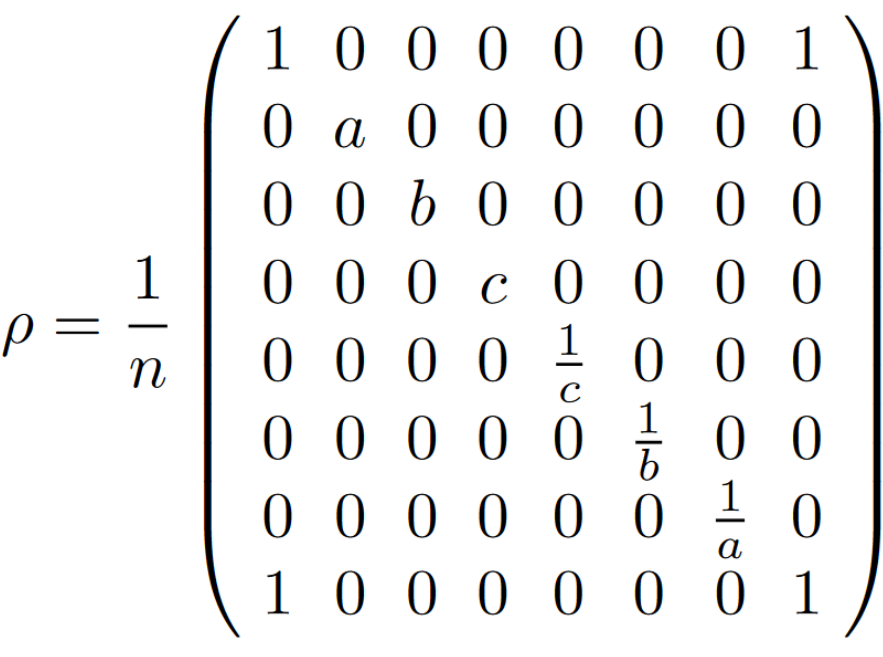
\includegraphics[width=\textwidth]{imgs/ppp.png}
    %\caption{}
    %\label{fig:}
\end{figure}

\end{minipage}



\phantom{42}

\onslide<2>{

Measure of entanglement: \textit{the logarithmic negativity}
\vspace{-3mm}
\begin{equation*}
    E_N = \log_2 (2 N_{AB} + 1), \vspace{-3mm}
\end{equation*}
with $N_{AB}$ is the absolute sum of the negative eigenvalues of $\rho_{AB}^{T_B}$.

}
} \frametitle{Entanglement witnesses: Peres-Horodecki criterion}}

% \frame{ %2Do: part transpose & PPTES, exp with corr on product
% \begin{tikzpicture}[overlay, remember picture]
    \node[anchor=north west, rotate=0, gray, font=\tiny, text width=\paperwidth] at (current page.south west)  [xshift=0, yshift=1.25cm] {
    [1] L. Amico et al., Entanglement in Many-Body Systems, Reviews of Modern Physics 80, no. 2 (2008)

    [2] A. Bergschneider et al., Experimental Characterization of Two-Particle Entanglement through Position and Momentum Correlations, Nature Physics 15, no. 7 (2019)
    };
\end{tikzpicture}

\only<1>{
\vspace{-7mm}
We can measure correlations: \vspace{-2mm}
\begin{figure}[h]
    \centering
    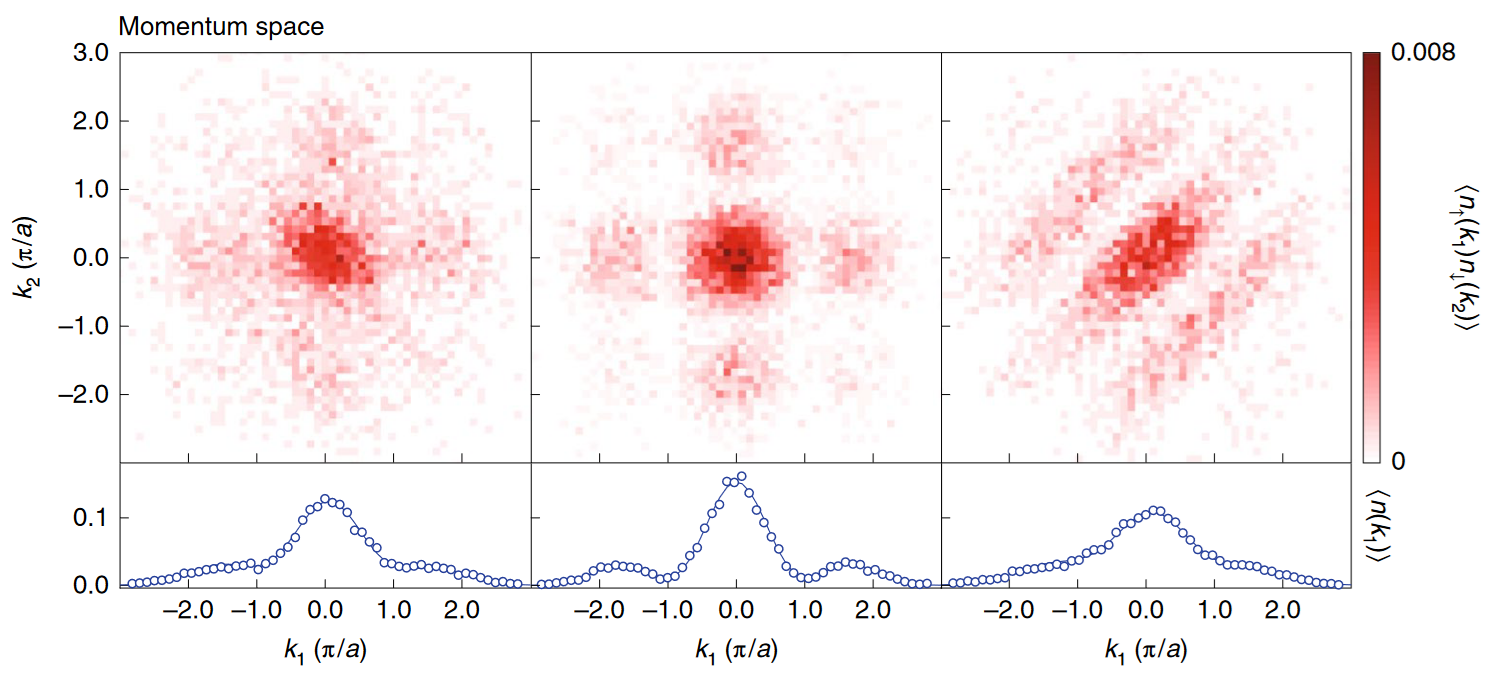
\includegraphics[width=0.75\textwidth]{imgs/eexp1.png}
    %\caption{}
    %\label{fig:}
\end{figure}
}

\only<2>{
\vspace{-7mm}
The pair correlators as entanglement witnesses: \vspace{-2mm}
    \begin{figure}[h]
        \centering
        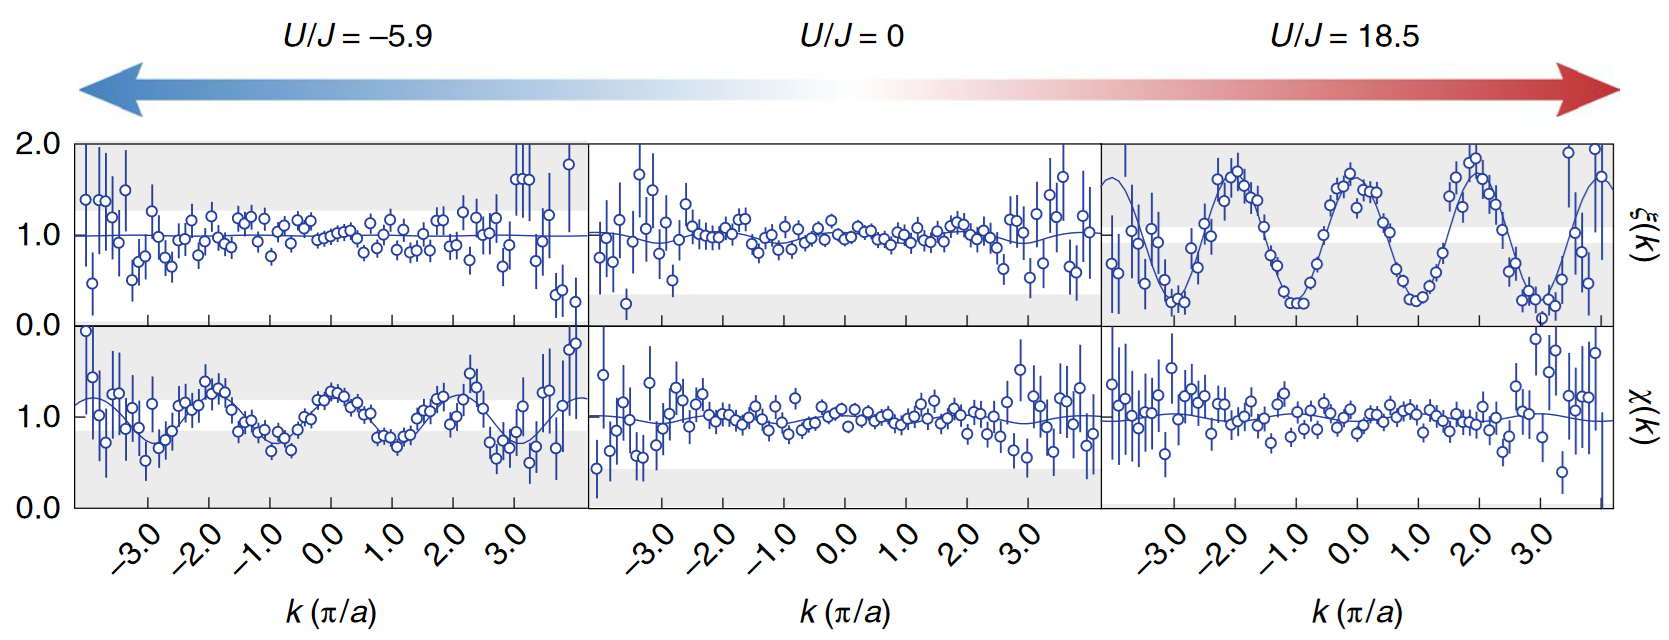
\includegraphics[width=0.9\textwidth]{imgs/eexp2.png}
        %\caption{}
        %\label{fig:}
    \end{figure}
    
}

\only<1>{
Construct the pair correlators \vspace{-3mm}
\begin{align*}
    \xi(d=k_1-k_2) &= \frac{
        \int d k\ \langle n_{\uparrow}(k-d/2) n_{\downarrow}(k+d/2)\rangle
    }{
        \int d k\ \langle n_{\uparrow}(k-d/2) \rangle \langle n_{\downarrow}(k+d/2)\rangle
    } 
    \\
    \chi(s=k_1+k_2) &= \frac{
        \int d k\ \langle n_{\uparrow}(k+s/2) n_{\downarrow}(-k+s/2)\rangle
    }{
        \int d k\ \langle n_{\uparrow}(k+s/2) \rangle \langle n_{\downarrow}(-k+s/2)\rangle
    } 
\end{align*}
}

\only<2>{

\phantom{42}

    For separable states: \vspace{-3mm}
    \begin{equation*}
         \sub{\xi}{min} \leq \xi  \leq \sub{\xi}{max},
         \hspace{5 mm} 
         \sub{\chi}{min} \leq \chi  \leq \sub{\chi}{max}.
    \end{equation*}
}
 \frametitle{Entanglement witnesses: example}}


% \frame{ %2Do
% \input{slides/loc.tex} \frametitle{Localizable entanglement}}


% \frame{ %2Do: как можно в общем случае измерить ренью энтропию
% \begin{tikzpicture}[overlay, remember picture]
    \node[anchor=north west, rotate=0, gray, font=\tiny, text width=0.65\paperwidth] at (current page.south west)  [xshift=0, yshift=1cm] {
    [5] A. Elben et al., Statistical Correlations between Locally Randomized Measurements, Physical Review A 99, no. 5 (2019)
    };
\end{tikzpicture}

\vspace{-7mm}
The second Rényi entropy \vspace{-3mm}
\begin{equation*}
	S_2 (\rho_A) = - \log_2 \tr \rho_A^2.
\end{equation*}



Bipartite entanglement exists between subsystems $A$ and $B$ of $\mathcal{S}$  with reduced density matrices $\rho_A = \tr_{\mathcal{S}\backslash A} \rho$ and $\rho_B = \tr_{\mathcal{S}\backslash B} \rho$ \textbf{if}
\begin{equation*}
	S_2 (\rho_A) > S_2 (\rho_{AB}) \hspace{5 mm} \text{or} \hspace{5 mm}  
	S_2(\rho_B) > S_2 (\rho_{AB}).
\end{equation*}

\begin{minipage}{0.65\textwidth}

\vspace{-5mm}
\begin{figure}[h]
    \centering
    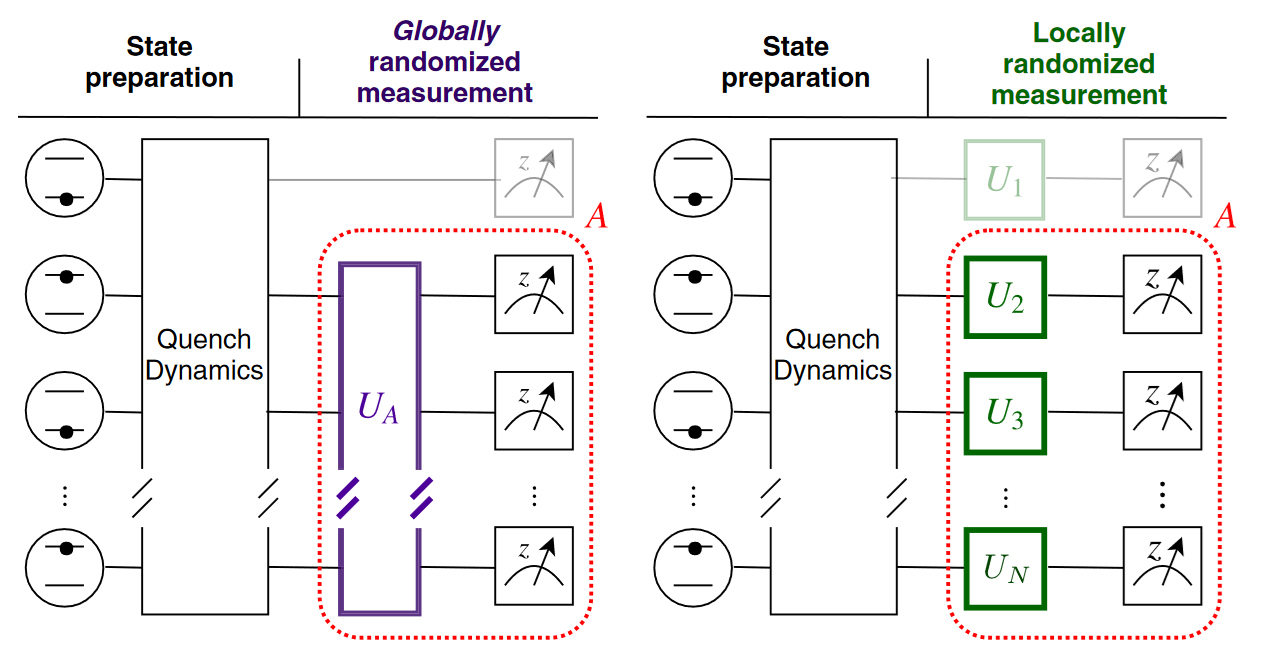
\includegraphics[width=\textwidth]{imgs/RU2.png}
    %\caption{}
    %\label{fig:}
\end{figure}


\end{minipage}
\hfill
\begin{minipage}{0.28\textwidth}
\begin{figure}[h]
    \centering
    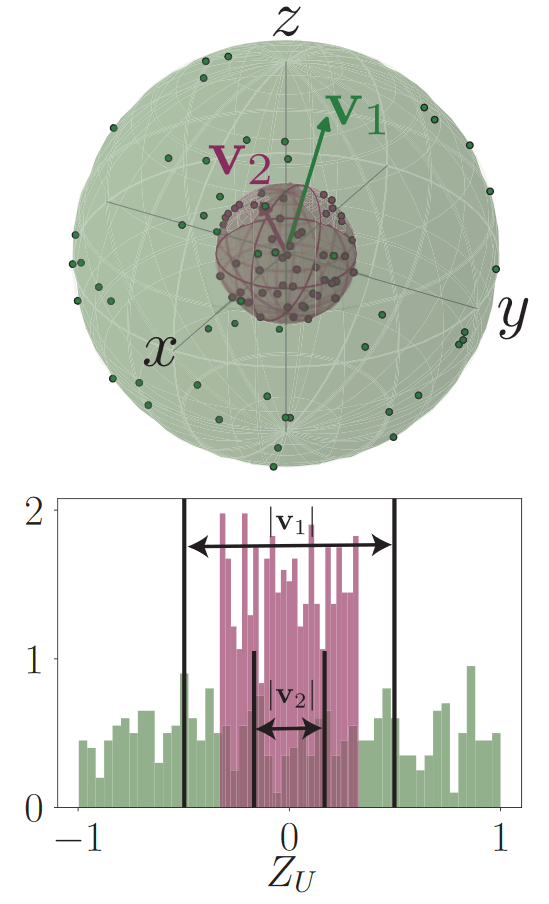
\includegraphics[width=\textwidth]{imgs/RU1.png}
    %\caption{}
    %\label{fig:}
\end{figure}
\end{minipage}


\onslide<2>{
\begin{tikzpicture}[overlay, remember picture]
    \fill[white,opacity=0.8] (current page.south west) rectangle (current page.north east);
    \node at (current page.center) {\usebeamerfont{title}\Huge\color{black} Thank you for your attention!};
\end{tikzpicture}
} \frametitle{Random Unitaries}}



\end{document}
